\documentclass{acm_proc_article-sp}
\usepackage{url}
\usepackage{algpseudocode}
\usepackage{verbatim}
\usepackage{microtype}
\usepackage{enumerate}
\usepackage{enumitem}
\usepackage{epsfig}
\usepackage{algorithmicx}
\usepackage{algorithm}
\usepackage{natbib}
\usepackage[utf8]{inputenc}
\begin{document}

\title{Similar Sentence Detection Using Locality Sensitive Hashing Technique on Wikipedia}

\numberofauthors{3}

\author{
\alignauthor Samet Ayhan\\
       \affaddr{University of Maryland}\\
       \affaddr{Dept. of Computer Science}
       \email{sayhan@cs.umd.edu}
\alignauthor Joshua Bradley\\
       \affaddr{University of Maryland}\\
       \affaddr{Dept. of Computer Science}
       \email{jgbrad1@cs.umd.edu}
\alignauthor Sarah E. Weissman\\
       \affaddr{University of Maryland}\\
       \affaddr{College of Information Studies}\\
       \email{sew@umd.edu}
}

\date{October 9, 2013}

\maketitle
\begin{abstract}
The growth of the Internet has enabled collaboration and cooperation on a large scale, resulting in an abundant number of near-duplicate web documents. Information is propagated on a large scale, which means that finding (and correcting) factual errors is made more difficult, since such errors may be duplicated many times over in different locations. Wikipedia articles, which are written and edited by an open community of mostly anonymous users are a prime candidate for copying of information. With few exceptions, the reader of any article can edit the text by copying from another article or an outside source without prior approval or confirmation of correctness. Although Wikipedia has its own policies and procedures for maintaining articles and improving quality, questions of the quality and accuracy of information on the website remain. Although we do not directy attempt to measure the quality of Wikipedia articles, we are interested in finding near-duplicate occurrences at various granularity levels. Such near duplicate sentences may reflect factual information that has been updated in one article and not another, or merely inconsistencies that should be flagged and addressed.

In this paper, we describe a similarity detection algorithm for Wikipedia articles that utilizes a locality sensitive hashing (LSH) technique on the MapReduce framework. The algorithm has been designed and implemented to detect similar content at the sentence level using large Wikipedia dumps. We also describe a heuristic method for classifying types of duplications on Wikipedia, which could be used for selecting and prioritizing editing efforts.
\end{abstract}

% A category with the (minimum) three required fields
\category{H.3.3}{Information Storage and Retrieval}[Information Search and Retrieval]

\terms{Algorithms, Design, MapReduce}

\section{Introduction}
The online encyclopedia Wikipedia is a collaboratively edited, multilingual, free resource. As of xxx date, it contains 26 million articles, over 4.2 million in English alone. These articles are written and edited by volunteer contributors around the world. Most articles can be edited by anyone with internet access, and there are currently approximately 100,000 active contributors.

Because of its open nature, Wikipedia has a history of generating controversy over editorial quality and factual correctness. Although some studies have found Wikipedia's accuracy to rival that of traditional encyclopedias, other studies have found numerous factual errors.[References??] Since Wikipedia may be edited anonymously, information may freely copied between web sources and even between Wikipedia articles without verification. Additionally, many articles in Wikipedia lack citations. Although there are active communities of editors who contribute to the upkeep of various articles, often focusing on a partiular subject area and expanding and improving the related content, still much of Wikipedia content is created in an unsupervised manner. Wilkinson found the distribution of article edits on Wikipedia to have a long tail, meaning that a small number of articles have many edits while most articles have few, and that the number of edits is directly related to article quality. Articles with low edits and low editorial attention, are less likely to be updated when new information is available \cite{wilkinson:wiki}.

Under such conditions, this type of large-scale collaborative effort may result in duplicate or near duplicate articles at various granular levels, such as sentence-level or multi-gram granularity \cite{wiki:weblink} [??]. For our purposes, we focus primarily on the sentence level. Near duplicate sentences may reflect factual information that has been updated in one article and not another (for example, information that varies over time, like populations or a country's GDP), or merely inconsistencies that should be flagged and addressed. 

Our approach applies minhashin, a well known, scalable, locality sensitive hashing (LSH) technique for near duplicate document detection. Since we are assuming the content we are looking for is not just similar, but has diverged due to an editorial process, as part of this work we investigate how well minhash approximates edit distance.  
We investigate the following questions:
\begin{itemize}[noitemsep,nolistsep]
\item How effectively does minhashing approximate edit distance? Edit distance seems like a reasonable metric for near duplicate sentences, however LSH does not map naturally to the edit distance metric.
\item How well do techniques for detecting near duplicate documents work when applied at the sentence level?
\item Do near duplicate sentences correspond to factual errors?
\end{itemize}

Along with these questions, we also considered the scalability and efficiency issues due to the large size of Wikipedia. To address these issues, we implemented our algorithm on the MapReduce computing framework.

The rest of this paper is organized as follows: In Section 2, we present related work, in Section 3, we explain the algorithm utilizing locality sensitive hashing, in Section 4, we discuss parameter tuning for Minhash. In Section 5, we present the working application within the MapReduce framework. In Section 6, we discuss our experiments with various Wikipedia datasets. The final section contains concluding remarks and future work.

\section{Related Work}
A number of techniques have been implemented to identify similarity between documents in the literature. These techniques usually differ in terms of corpus of interest, signature representing the document, feature-set determined by the system, and the end goal of the analysis.

Broder et al. introduced shingling to compute document similarity and containment. They also presented methods for using a subset of shingles while still allowing similarity and containment computations \cite{broder:resemblance}.

Seo et al. defined a general framework for text reuse detection. They introduced Discrete Cosine Transform (DCT) fingerprinting for general or local text reuse detection with high accuracy and efficiency \cite{seo:dct}.

Zhang et al. presented partial duplicate detection algorithm using sequence matching that transforms partial-duplicate detection task into three MapReduce jobs: 1.Indexing, 2.Sequence Duplicate Detection, 3.Sequence Matching \cite{zhang:pdc}.

Hajishirzi et al. introduced an adaptive near-duplicate detection (ANDD) method by extending term-weighting framework to learn k-gram vectors. Provided that each document was represented by an informative real k-gram vector, similarity measures were computed to come up with predicted values of near-duplicates \cite{hajishirzi:andd}.

Lin described three MapReduce algorithms for computing pairwise similarity on document collections \cite{lin:brute}.
\begin{enumerate}[noitemsep,nolistsep]
\item Based on brute force.
\item Treated as large-scale ad hoc retrieval.
\item Based on Cartesian product of postings lists.
\end{enumerate}

Manku et al. used Charikar's fingerprinting technique for developing near-duplicate detection system. They presented an algorithmic technique for identifying existing f-bit fingerprints that differ from a given fingerprint in at most k bit-positions, for small k. They demonstrated that their system is useful not only for batch but also for online processing \cite{manku:web}.

Bendersky et al. examined two information flow representations: the timeline and the link graph. They proposed several simple unsupervised techniques for timeline construction link graph analysis \cite{bendersky:timeline}.

In order to handle large Wikipedia dumps with the order of tens or hundreds of gigabytes and even a few terabytes, we used MapReduce framework in this work, that was introduced by Dean and Ghemawat \cite{dean:mapreduce}. 

\section{Algorithm Utilizing Locality \\ Sensitive Hashing}

In order to measure document similarity we use a common LSH technique known as MinHash (\cite{broder:resemblance}). A minhash signature on a text document is calculated using a parametrized family of hash functions $F_i$, $1 \le i \le N$. (In our case, input ''documents'' are individual sentences found within the content of Wikipedia articles.) Each document is broken up into n-gram ``shingles'' and for each shingle set $S$ a set $\{min_{s \in S}(F_i(s)\}$ of minimum hashes over the hash family is produced. The signature on a document $d$ is represented as a vector of $K$ minhashes, chosen from the set $\{min_{s \in S}(F_i(s)\}$ of minimum hashes. In order to minimize false negatives we apply a technique sometimes known as ``banding'' \cite{ullman:massive} where multiple signatures are produced for each input document.

\subsection{Design}
Many signature techniques such as LSH are embarrassingly parallel. In our project, we designed our algorithm around the MapReduce framework.

Because the minhash technique is parametrized by several variables, including shingle length, signature size, and number of signatures to be calculated per document, these values can also be considered as inputs for the MapReduce algorithm.

\begin{table}
\begin{algorithm}[H]
\caption{Minhash MapReduce Pseudocode}
\begin{algorithmic}
\Function{initialize}{}
%\Comment{configure and set up algorithm parameters}
 \State $F \gets $ hash family;
 \State $L \gets $ shingle length;
 \State $K \gets $ vector length;
 \State $N \gets $ number of signatures to emit;
\EndFunction

\Function{map}{docid $d$, wikipage $p$}
 \State sentencect $\gets 0$
 %\Comment {Break up article text into sentence}
 \While{$s \gets$ nextSentence($p$)}
  %\Comment{Break up sentence into shingles}
  \State shingles $\gets$ shingleSet($s$,$L$);
  \State minhashes = new List(|F|);
   \For{$i \gets 1 \ldots |F|$}
    \State minhashes[$i$] $\gets \infty$;
   \EndFor
   %\Comment{Calculate set of minhash signature for each sentence}
   \For{$g \in$ shingles}
    \For{$i \gets 1 \ldots |F|$}
     \State minhashes[$i$] $\gets$ min($F_i(g)$,minhashes[$i$]);
    \EndFor
   \EndFor
   %\Comment{Emit $N$ $K$-length signatures}
  \For{$i \gets 1 \ldots N$}
   \State sig = select($K$, minhahses);
   \State emit(sig,(docid,sentencect));
  \EndFor
  \State  sentencect++;
 \EndWhile
\EndFunction

\Function{reduce}{signature sig, sentenceids $S$}
\If{$|S| > 1$}
\State emit(sig, $S$);
\EndIf
\EndFunction
\end{algorithmic}
\end{algorithm}
\end{table}

\subsection{Implementation Details}

Our implementation is built on top of the Apache Hadoop MapReduce framework, using utilities from the Cloud9 (\url{https://github.com/lintool/Cloud9}) and WikiClean (\url{https://github.com/lintool/wikiclean/}) libraries for parsing Wikipedia page text from the Wikipedia XML dump format. An open source implementationis available on Github (\url{https://github.com/seweissman/wikiduper}).

%Sentences are parsed out over each document using a regular expression. Sentences that are too large or too small are discarded. The family of hash functions is implemented using a ``Multiply Shift'' (\url{http://en.wikipedia.org/wiki/Universal_hashing}) hashing scheme and is generated from a random seed using the Java Random class. The hash family is also parametrized by hash output key size and this value can be configured to affect the size of the output signatures.

\section{Parameter Tuning}

As mentioned above the minhash algorithm is parametrized by several values, including shingle length, length of hash vectors, number of hash bands, and hash output size. Each of these parameters has an impact on the error rates in the minhash output. 

\subsection{Jaccard Similarity and Edit Distance}

%Jaccard similarity is a measure of set similarity while our stated goal is to find sentences in Wikipedia that have been copied from one article to another and possibly edited. A more natural measure to use for this application is edit distance, but there is no known good locality sensitive hashing family for edit distance \cite{Kirsch06distance-sensitivebloom}.

In order to estimate Jaccard similarity of sentences $X$ and $Y$ in terms of edit distance we assume that $X$ and $Y$ are both of length $N$ and that their shingle sets are of maximum size (i.e. all shingles are unique). Also assume that $X$ and $Y$ have edit distance $e$.  We limit type of edits to changing characters in place. Additionally, to simplify our calculations, we assume that edits are localized so that no shingle overlaps more than one edit.

(WLOG) Let $S$ be the set of shingles for X and let $S_o$ be the set of shingles of X that overlap edits. The maximum number of unique shingles for a sentence of length $N$ is $N - L + 1 = |S|$. Also, we can see that $e \le |S_o| \le e + L - 1$. Since edits at the start or end of the sentence will overlap with fewer shingles than edit mid-sentence.

Now we can define $|X \cup Y|$ and $|X \cap Y|$ in terms $S$ and $S_o$ as follows:
\begin{eqnarray*}
|X \cap Y| & = & |S| - |S_o| \\
|X \cup Y| & = & 2*|S_o| + |X \cap Y| \\
           & = & |S_o| + |S|
\end{eqnarray*}

Plugging in the values above for $|S_o|$ and $|S|$ we get:

\begin{eqnarray*}
E + N - L + 1  \le & |X \cup Y| & \le E + N \\
N - L + 1 - E  \ge & |X \cap Y| & \ge N - 2L - E + 2 \\
\end{eqnarray*}
\begin{eqnarray*}
\frac{N - L - E + 1 }{N - L + e + 1} >= & J(X,Y) & >= \frac{N - 2L - E + 2}{N + E}
\end{eqnarray*}

Note that, at least under this set of assumptions, the Jaccard similarity is always less than the ``edit similarity'' (1 - normalized edit distance):

\begin{eqnarray*}
J(X,Y) & <= & \frac{N - E}{E + N - L + 1} - \frac{L - 1}{E + N - L + 1} \\
       & <= & \frac{N - E}{N} \\ 
       & =  & 1 - \frac{E}{N}
\end{eqnarray*}

Finally we can divide through the equations for J(X,Y) by N, which gives us:

\begin{eqnarray*}
\frac{1 - l - e}{1 - l + e} >= J(X,Y) >= \frac{1 - 2l - e}{1 + e}
\end{eqnarray*}

where $l$ is relative shingle size and $e$ is normalized edit distance.

Note that as relative shingle size goes to 0 there is a nice convergence for Jaccard similarity:
\[\lim_{l->0}J(X,Y) = \frac{1 - e}{1 + e}\]

\begin{figure}
\centering
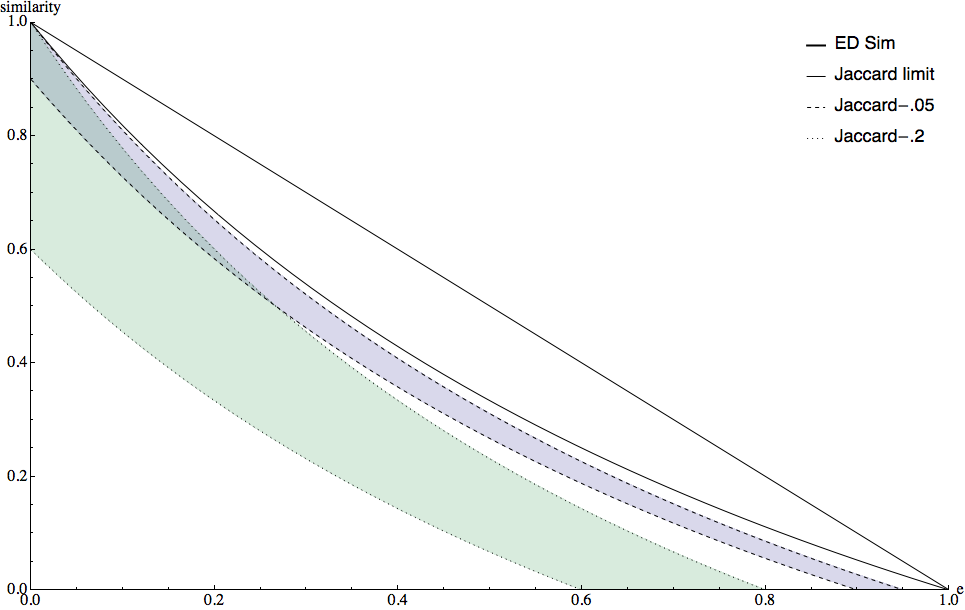
\includegraphics[width=3.5in, keepaspectratio = true]{jac-ed-chart.png}
\caption{Jaccard Similarity vs. normalized edit distance.}
\label{jac-ed}
\end{figure}

As we would expect, Jaccard similarity decreases as edit distance increases, but it also decreases as shingle length increases. Figure \ref{jac-ed} shows Jaccard Similarity plotted against edit distance for $l = .05$ and $l = .2$. At $l = .05$ and $e = .2$ our estimate for Jaccard similarity has already fallen to the range [0.58,0.65]. Clearly setting $l$ too high can increase the false positive rate, but setting $l$ too low will increase the false positive rate, since it will increase the size of the intersection of the shingle sets.

\subsection{False positives}

In order to estimate the affect of shingle length on false positive rate we ran a number of experiments for a 1 G collection of wikipedia documents. For fixed $N=10$ we ran experiments for three values of $K=\{8,9,10\}$ and $8 \le L \le 16$. Setting a normalized edit distance threshold of $e = .25$, we calculated the total number of ''good'' ($e <= .25$) and ''bad'' ($e > .25$) (unique) sentence pairs as well as the false positive rate (\# bad pairs divided by the total number of sentences). Results are presented in Figure \ref{ed-grid}.

As we might expect, as shingle length increases, the false positive rate decreases. However, the total number of good pairs also decreases, implying that our false negative rate is also increasing. When applying these techniques, increased recall will come at the price of decreased precision. Because of this, in a real implementation, it would likely be desirable to set requirements for recall, then use secondary filtering to increase precision. For example, actual edit distance could be applied as a secondary filter.

\begin{figure}
\centering
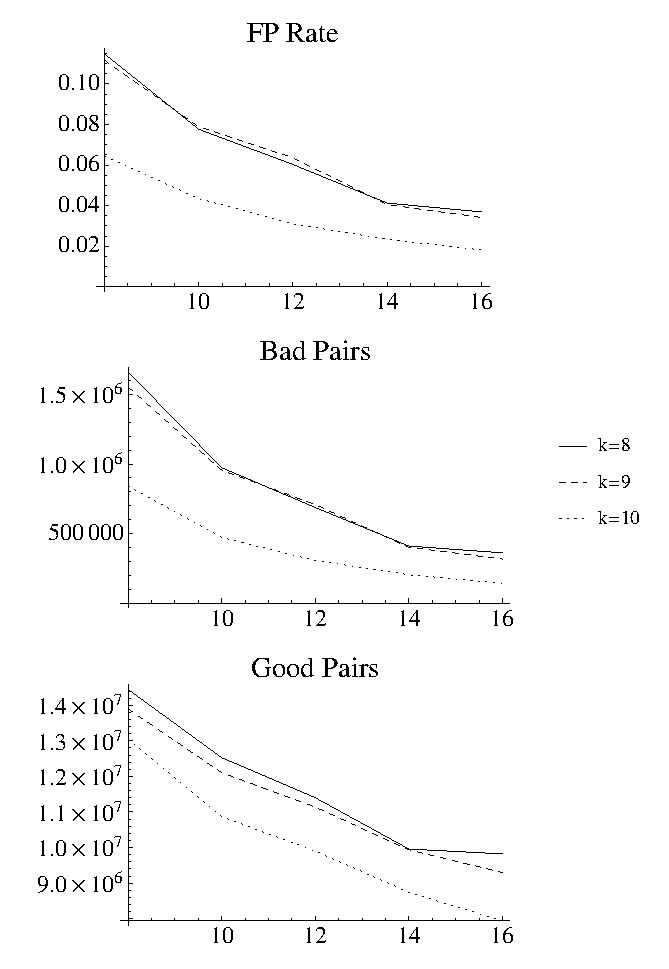
\epsfig{file=edgridl.eps,width=3.5in}
\caption{False Positive Rate, Good Count, Bad Count for $N=10, K \in \{8,9,10\}, 5 \le L \le 15$}
\label{ed-grid}
\end{figure}

\section{Experiments and Discussion}

%We performed several analyses to provide more insight into the occurence of duplicate sentences. In particular, we were interested in detecting similar sentences that arose from copying text from one article to another since such instances would represent content that is either redundant, or content that has diverged in the sense that either the original or the copy was edited for clarification of factual correctness and the other was not. Such instances give insight into the Wikipedia editing process, and also represent an opportunity to improve article quality on Wikipedia by identifying places where further editing or article merging may be needed.

All of our experiments were run against an XML dump of current English-language Wikipedia (enwiki) articles (as of 7/2013) obtained from dumps.wikimedia.org. The enwiki dump is approximately 42G in size and contains 10,218,778 articles (after excluding certain non-article page types). Running our application on the enwiki dump on a shared cluster of 16 nodes (20 GB RAM and 4? cores each) took $\approx$ 25 minutes.

The total number of similar sentence clusters was 1,151,640, including 3,496,074 article/sentence pairs over 1,091,804 article titles. The total number of unique sentences over all clusters was 2,361,886.

Cluster sizes ranged from 2 to 42,901. (See Figure \ref{clust} for a breakdown of counts by cluster size.) Most sentence clusters are small, about 99\% of our clusters have size below or equal to 10, but about 1/4 of the output sentence/article pairs fall into clusters with size greater than 10. One explanation for this distribution of sentences is the phenomenon we call ''templatification,'' which we describe in more detail below.

\begin{figure}
\centering
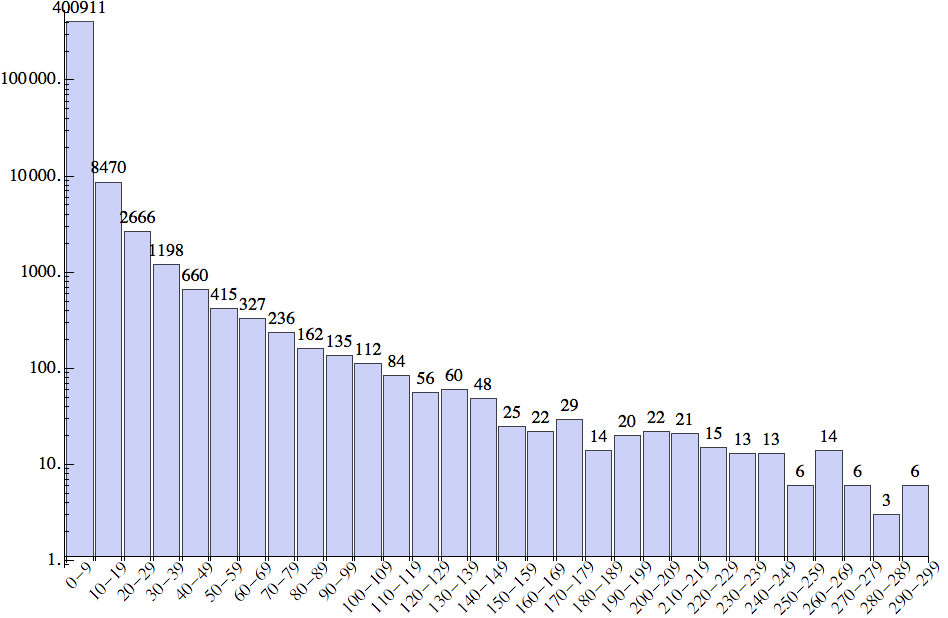
\includegraphics[width=3.5in, keepaspectratio = true]{clusterhistogram.png}
\caption{Histogram of Cluster Sizes (for cluster size $< 300$, log scale).}
\label{clust}
\end{figure}

\subsection{Similar Sentence Types}

Manual inspection of cluster output reveals several different similar sentence types. These types can be summarized as follows:

\begin{itemize}
\item Templatification
\item References
\item Direct Copying
\item Direct Copying with Copy Editing
\item Direct Copying with Factual Drift
\end{itemize}

 \emph{Templatification} occurs when one sentence is an exact duplicate of another sentence, but the main topic has been changed by only a few pieces of key information having been modified. For example, it could be said that the following two sentences follow a particular \emph{template}.
\begin{itemize}[noitemsep,nolistsep]

\item Of the agricultural land 40.4\% is used for growing crops and 26.6\% is pastures while 2.2\% is used for orchards or vine crops. [Gondiswil]
\item Of the agricultural land 26.1\% is used for growing crops and 30.2\% is pastures while 3.0\% is used for orchards or vine crops. [Kleindietwil]
\item Of the agricultural land 37.8\% is used for growing crops and 35.5\% is pastures while 2.2\% is used for orchards or vine crops. [Leimiswil]

\end{itemize}
From the perspective of editing/writing Wikipedia articles, this is a strong indicator that the author copied the original sentence and modified the relevant information to pertain to a different topic. What remains shared between both sentences though is the inherent structure.

\emph{Direct Copying} occurs when the same sentence has been copied into another (or possibly the same) article. This can happen for many reasons, including articles that deal with similar subjects, or articles that are subtopics of other topics Similarly, \emph{Direct Copying with Copy Editing} occurs when the same sentence has been copied into another article and then one or both sentences has been edited for style or clarity. For example:
\begin{itemize}[noitemsep,nolistsep]
\item In dry areas it may only emerge from its burrow for a few weeks when conditions are right and usually at night but in areas with permanent water bodies and abundant rain it may be active all day. [Great Plains toad]
\item In dry areas it may only emerge from its burrow for a few weeks when conditions are right and only at night but in areas with permanent water bodies and abundant rain it may be active all day. [List of amphibians and reptiles of Montana]
\end{itemize}

\emph{Factual drift} most notably occurs when the same sentence has been copied and a piece of factual information about the \emph{same} topic has changed. For example, factual drift can be seen in the following two sentences.
\begin{itemize}[noitemsep,nolistsep]
\item The color of the upper rim of an astronomical object could go from green to blue to violet depending on the decrease in concentration of pollutants as they spread throughout an increasing volume of atmosphere. [Green flash]
\item The color of the upper limb of an astronomical object could go from blue to green to violet depending on the decrease in concentration of pollutants as they spread throughout an increasing volume of atmosphere. [Mirage of astronomical objects]
\end{itemize}
Although factual drift is similar to copy editing and may occur along with copy editing, we distinguish the two cases since factual errors are more severe than style issues.

\emph{References} refers to citations, typically occurring at the end of a Wikipedia article. Since Wikipedia does not adhere to one single citation style, the same work may be referenced on multiple pages in different styles. Similarly different portions of the same work may be referenced in different articles. Although citation errors might be harder to distinguish from factual errors, errors in citation are arguably no less important. (It would also be interesting to compare whether articles that share similar sentences also share similar citations.) 

\begin{itemize}[noitemsep,nolistsep]
\item Neotropical Ichthyology 11 (1): 73-80.
\item Neotropical Ichthyology 10 (2): 245-253.
\end{itemize}

\subsubsection{Break down of sentence types}

By manually counting a small sample of 2094 output clusters, we came up with a breakdown of sentence types shown in Table \ref{counts}.

\begin{table}
\centering
\caption{Sentence Breakdown Counts}
\begin{tabular}{| l | c | c |}
\hline
Factual Drift & 121 & 5.78\% \\ \hline
Template & 632 & 30.18\% \\ \hline
Reference & 7 & 0.33\% \\ \hline      
Copy Edit & 283 & 13.51\% \\ \hline
Identical & 948 & 45.27\% \\ \hline
Other & 103 & 2.92\% \\ \hline
\hline
\end{tabular}
\label{counts}
\end{table}

To get a rough estimate of the number of template clusters, we develop a heuristic score on low frequency words in the cluster word set to identify templates. For our purposes a low-frequency word is one that occurs in less than half of the cluster sentences. The score we use is:
\[(\#numeric + \#proper)/(\#numeric + \#proper + \#other)\]
Where \#numeric is the number of numeric terms in the cluster word set (all unique words occuring in the cluster), \#proper is the number of proper nouns in the cluster word set (i.e. capitalized words), and \#other is the number of other words.

Applying the score to our hand-classified clusters shows us that this score does separate between template and non-template clusters. (Everything that isn't in the Template class is considered a non-Template for the binary classification exercise.) See Figure \ref{heuristic}.

After applying the score to the entire set of wiki clusters (with a score threshold of .6), there are 244,660 template clusters and 906,960 non-template clusters, including 666,212 identical clusters. The template clusters contain 1,116,932 sentences, and the non-template clusters contain 1,244,196 sentences.

\begin{figure}
\centering
\includegraphics[width=3.5in, keepaspectratio = true]{classifyscoreswikinew.pdf}
\caption{Histogram of Hand Labeled Clusters by Template Heuristic Score.}
\label{heuristic}
\end{figure}


\subsection{Sentence Similarity as a Measure of Article Similarity}

\begin{figure}
\begin{center}
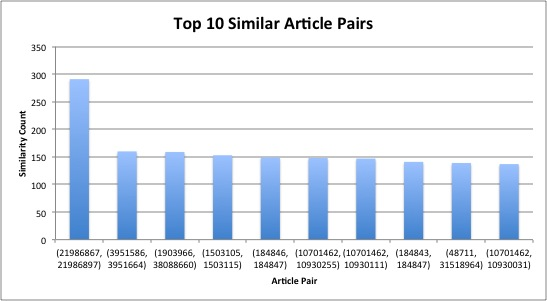
\includegraphics[scale=0.43, keepaspectratio = true]{Top10ArticlePairs.jpg}
\end{center}
\caption{Top 10 Similarity Counts}
\label{toparticles}
\end{figure}

 For clarity purposes, we define \emph{similarity count} as simply the total number of sentences between two articles that were found to share the same hash signature. Using the output of the minhashing routine, we performed a pairwise similarity count across all articles that shared similar sentences. Overall, we found $\approx 29580$ wikipedia article pairs that had a similarity count greater than $50$.

Looking at the distribution of cluster sizes in Figure \ref{clust}, we can see the expected behavior of decreasing number of clusters of size $k$ as $k$ grows large. What is unusual though is the number of relatively large clusters in the size range of $[25, 65]$. Based on the fact that we found $\approx 6500$ article pairs with a similarity count greater than $50$, this would indicate that there are collections of articles that have a large number of near-duplicate sentences in common. As can be seen in the Top 10 similarity counts, there can even be chains of articles that share large portions of their content with each other (a chain of 3 is demonstrated in Figure \ref{toparticles}).

\begin{table}
\centering
\caption{Top 10 Article Pair Titles}
{\small
\begin{tabular}{| l |}
    \hline
\{Private equity in the 2000s, History of private equity and venture capital, Private equity in the 1980s\} \\
\{List of ethnic cleansings, Ethnic cleansing\} \\
\{Route of the Oregon Trail, Oregon Trail\} \\
\{English literature, British literature\} \\
\{Portia schultzi, Portia labiata, Portia fimbriata\} \\
\{Lesbian American history, List of lesbian, gay, bisexual, or transgender firsts by year\} \\
\{Lists of British inventions, List of English inventions and discoveries\} \\
\{1981 in baseball, 1981 Major League Baseball season\} \\
\{Minority Report (film), Themes in Minority Report\} \\
\{What Is History?, E. H. Carr\} \\
\{Individualist anarchism in Europe, Individualist anarchism in the United States, Individualist anarchism, Anarchism in the United States\} \\
\{Kingdom of Scotland, Scotland in the Early Modern Era\} \\
\{Decline of Greco-Roman polytheism, Christian persecution of paganism after Theodosius I until the fall of the Roman Empire\} \\
\{Anarchist schools of thought, Libertarian socialism, Anarchist communism, Anarchism, History of anarchism, Libertarian Marxism\} \\
\{Brill Tramway, Quainton Road railway station\} \\
\{History of the Roman Empire, Byzantine Empire, History of the Byzantine Empire\} \\
\{List of American state and local politicians convicted of crimes, List of state and local political scandals in the United States\} \\
\{Filioque, History of the Filioque controversy\} \\
\{1960 Major League Baseball season, 1960 in baseball\} \\
\{Domitian, Flavian dynasty\} \\
\{Military history of Australia during World War II, Australian Army during World War II\} \\
\{Kuomintang, History of the Kuomintang\} \\
\{Interracial marriage, Miscegenation, Eurasian (mixed ancestry)\} \\
\{Scotland in the modern era, History of Scotland\} \\
\{History of California, Maritime history of California\} \\
\{Outline of project management, Glossary of project management\} \\
\{Wigan Warriors, History of Wigan Warriors\} \\
\{List of American federal politicians convicted of crimes, List of federal political scandals in the United States\} \\
\{Economy of England in the Middle Ages, Economics of English towns and trade in the Middle Ages\} \\
\{Galvatron, Megatron\} \\
\{Metropolitan Police role in the news media phone hacking scandal, News media phone hacking scandal\} \\
\{List of Shakespearean characters (L-Z), List of Shakespearean characters (A-K), List of historical figures dramatised by Shakespeare\} \\
\{Fetal alcohol spectrum disorder, Fetal alcohol syndrome\} \\
\{List of marine bony fishes of South Africa, List of marine animals of the Cape Peninsula and False Bay\} \\
\{History of painting, Western painting, 20th-century Western painting\} \\
\{Timeline of the 2007 Burmese anti-government protests, 2007 Burmese anti-government protests\} \\
\{Precipitation, Rain\} \\
\{List of Puerto Ricans, List of Puerto Rican military personnel\} \\
\{Glossary of basketball terms, Outline of basketball\} \\
\{Hannibal, Conquests of Hannibal\} \\
\{Bogotá, History of Bogotá\} \\
\{Pseudotsuga menziesii var. menziesii, Douglas fir\} \\
\{History of the East-West Schism, East-West Schism\} \\
\{List of attacks in Lebanon, Lebanon bombings and assassinations (2004-present)\} \\
\{Zen, Chinese Chán\} \\
\{List of Deadliest Warrior episodes, Deadliest Warrior (season 1), Deadliest Warrior (season 3), Deadliest Warrior (season 2)\} \\
\{1991 Major League Baseball season, 1991 in baseball\} \\
\{American rock, Rock music\} \\
\{Test matches in England in 2005, Australian cricket team in England in 2005\} \\
\{Swedes, Sweden\} \\
\{Glossary of robotics, Outline of robotics\} \\
\{CIA leak scandal criminal investigation, Plame affair grand jury investigation\} \\
\{History of Australia since 1945, History of Australia\} \\
\{List of Russian people, List of Russian scientists\} \\
    %% 21986867 & 2000 New Year Honours \\ \hline
    %% 21986897 & 1999 New Year Honours \\ \hline
    %% 3951586 & Instruments of the United Kingdom, 1994 \\ \hline
    %% 3951664 & Instruments of the United Kingdom, 1995 \\ \hline
    %% 1903966 & Management of baldness \\ \hline
    %% 38088660 & Management of androgenic alopecia \\ \hline
    %% 1503105 & Jayne Torvill \\ \hline
    %% 1503115 & Christopher Dean \\ \hline
    %% 184843 & Henry VI, Part 1 \\ \hline
    %% 184846 & Henry VI, Part 2 \\ \hline
    %% 184847 & Henry VI, Part 3 \\ \hline
    %% 10701462 & List of birds of Zambia \\ \hline
    %% 10930255 & List of birds of Zimbabwe \\ \hline
    %% 10930111 & List of birds of Mozambique \\ \hline
    %% 48711 & Oregon Trail \\ \hline
    %% 31518964 & History of the Oregon Trail \\
    \hline
\end{tabular}
}
\end{table}


\section{Conclusion and Future Work}
This paper presents our work on near-duplicate detection of Wikipedia articles at the sentence-granularity level using MinHash, a LSH technique. Our novel MapReduce algorithm tackles the problem by transforming it into more manageable pieces where each piece is handled in parallel. Our unique contribution includes empirical analysis of signatures belonging to Wikipedia articles at the sentence level. Experimental results verify that the proposed method is able to effectively and efficiently detect similar articles.

In the future, we would like to investigate revision histories of these articles, correlate them with their timestamps, and better relate similarities based on temporal dimensions. 

\section{Acknowledgments}
We would especially like to thank Dr. Jimmy Lin for his advise and directions.

\bibliographystyle{abbrv}
\bibliography{sigproc}  % sigproc.bib is the name of the Bibliography in this case

\balancecolumns
\end{document}
